\documentclass[11pt,a4paper]{report}
\usepackage[textwidth=37em,vmargin=30mm]{geometry}
\usepackage{calc,xunicode,amsmath,amssymb,paralist,enumitem,tabu,booktabs,datetime2,xeCJK,xeCJKfntef,listings}
\usepackage{tocloft,fancyhdr,tcolorbox,xcolor,graphicx,eso-pic,xltxtra,xelatexemoji}

\newcommand{\envyear}[0]{2025}
\newcommand{\envdatestr}[0]{2025-01-03}
\newcommand{\envfinaldir}[0]{webdb/2025/20250103/final}

\usepackage[hidelinks]{hyperref}
\hypersetup{
    colorlinks=false,
    pdfpagemode=FullScreen,
    pdftitle={Web Digest - \envdatestr}
}

\setlength{\cftbeforechapskip}{10pt}
\renewcommand{\cftchapfont}{\rmfamily\bfseries\large\raggedright}
\setlength{\cftbeforesecskip}{2pt}
\renewcommand{\cftsecfont}{\sffamily\small\raggedright}

\setdefaultleftmargin{2em}{2em}{1em}{1em}{1em}{1em}

\usepackage{xeCJK,xeCJKfntef}
\xeCJKsetup{PunctStyle=plain,RubberPunctSkip=false,CJKglue=\strut\hskip 0pt plus 0.1em minus 0.05em,CJKecglue=\strut\hskip 0.22em plus 0.2em}
\XeTeXlinebreaklocale "zh"
\XeTeXlinebreakskip = 0pt


\setmainfont{Brygada 1918}
\setromanfont{Brygada 1918}
\setsansfont{IBM Plex Sans}
\setmonofont{JetBrains Mono NL}
\setCJKmainfont{Noto Serif CJK SC}
\setCJKromanfont{Noto Serif CJK SC}
\setCJKsansfont{Noto Sans CJK SC}
\setCJKmonofont{Noto Sans CJK SC}

\setlength{\parindent}{0pt}
\setlength{\parskip}{8pt}
\linespread{1.15}

\lstset{
	basicstyle=\ttfamily\footnotesize,
	numbersep=5pt,
	backgroundcolor=\color{black!5},
	showspaces=false,
	showstringspaces=false,
	showtabs=false,
	tabsize=2,
	captionpos=b,
	breaklines=true,
	breakatwhitespace=true,
	breakautoindent=true,
	linewidth=\textwidth
}






\newcommand{\coverpic}[2]{
    % argv: itemurl, authorname
    Cover photo by #2~~(\href{#1}{#1})
}
\newcommand{\makeheader}[0]{
    \begin{titlepage}
        % \newgeometry{hmargin=15mm,tmargin=21mm,bmargin=12mm}
        \begin{center}
            
            \rmfamily\scshape
            \fontspec{BaskervilleF}
            \fontspec{Old Standard}
            \fontsize{59pt}{70pt}\selectfont
            WEB\hfill DIGEST
            
            \vfill
            % \vskip 30pt
            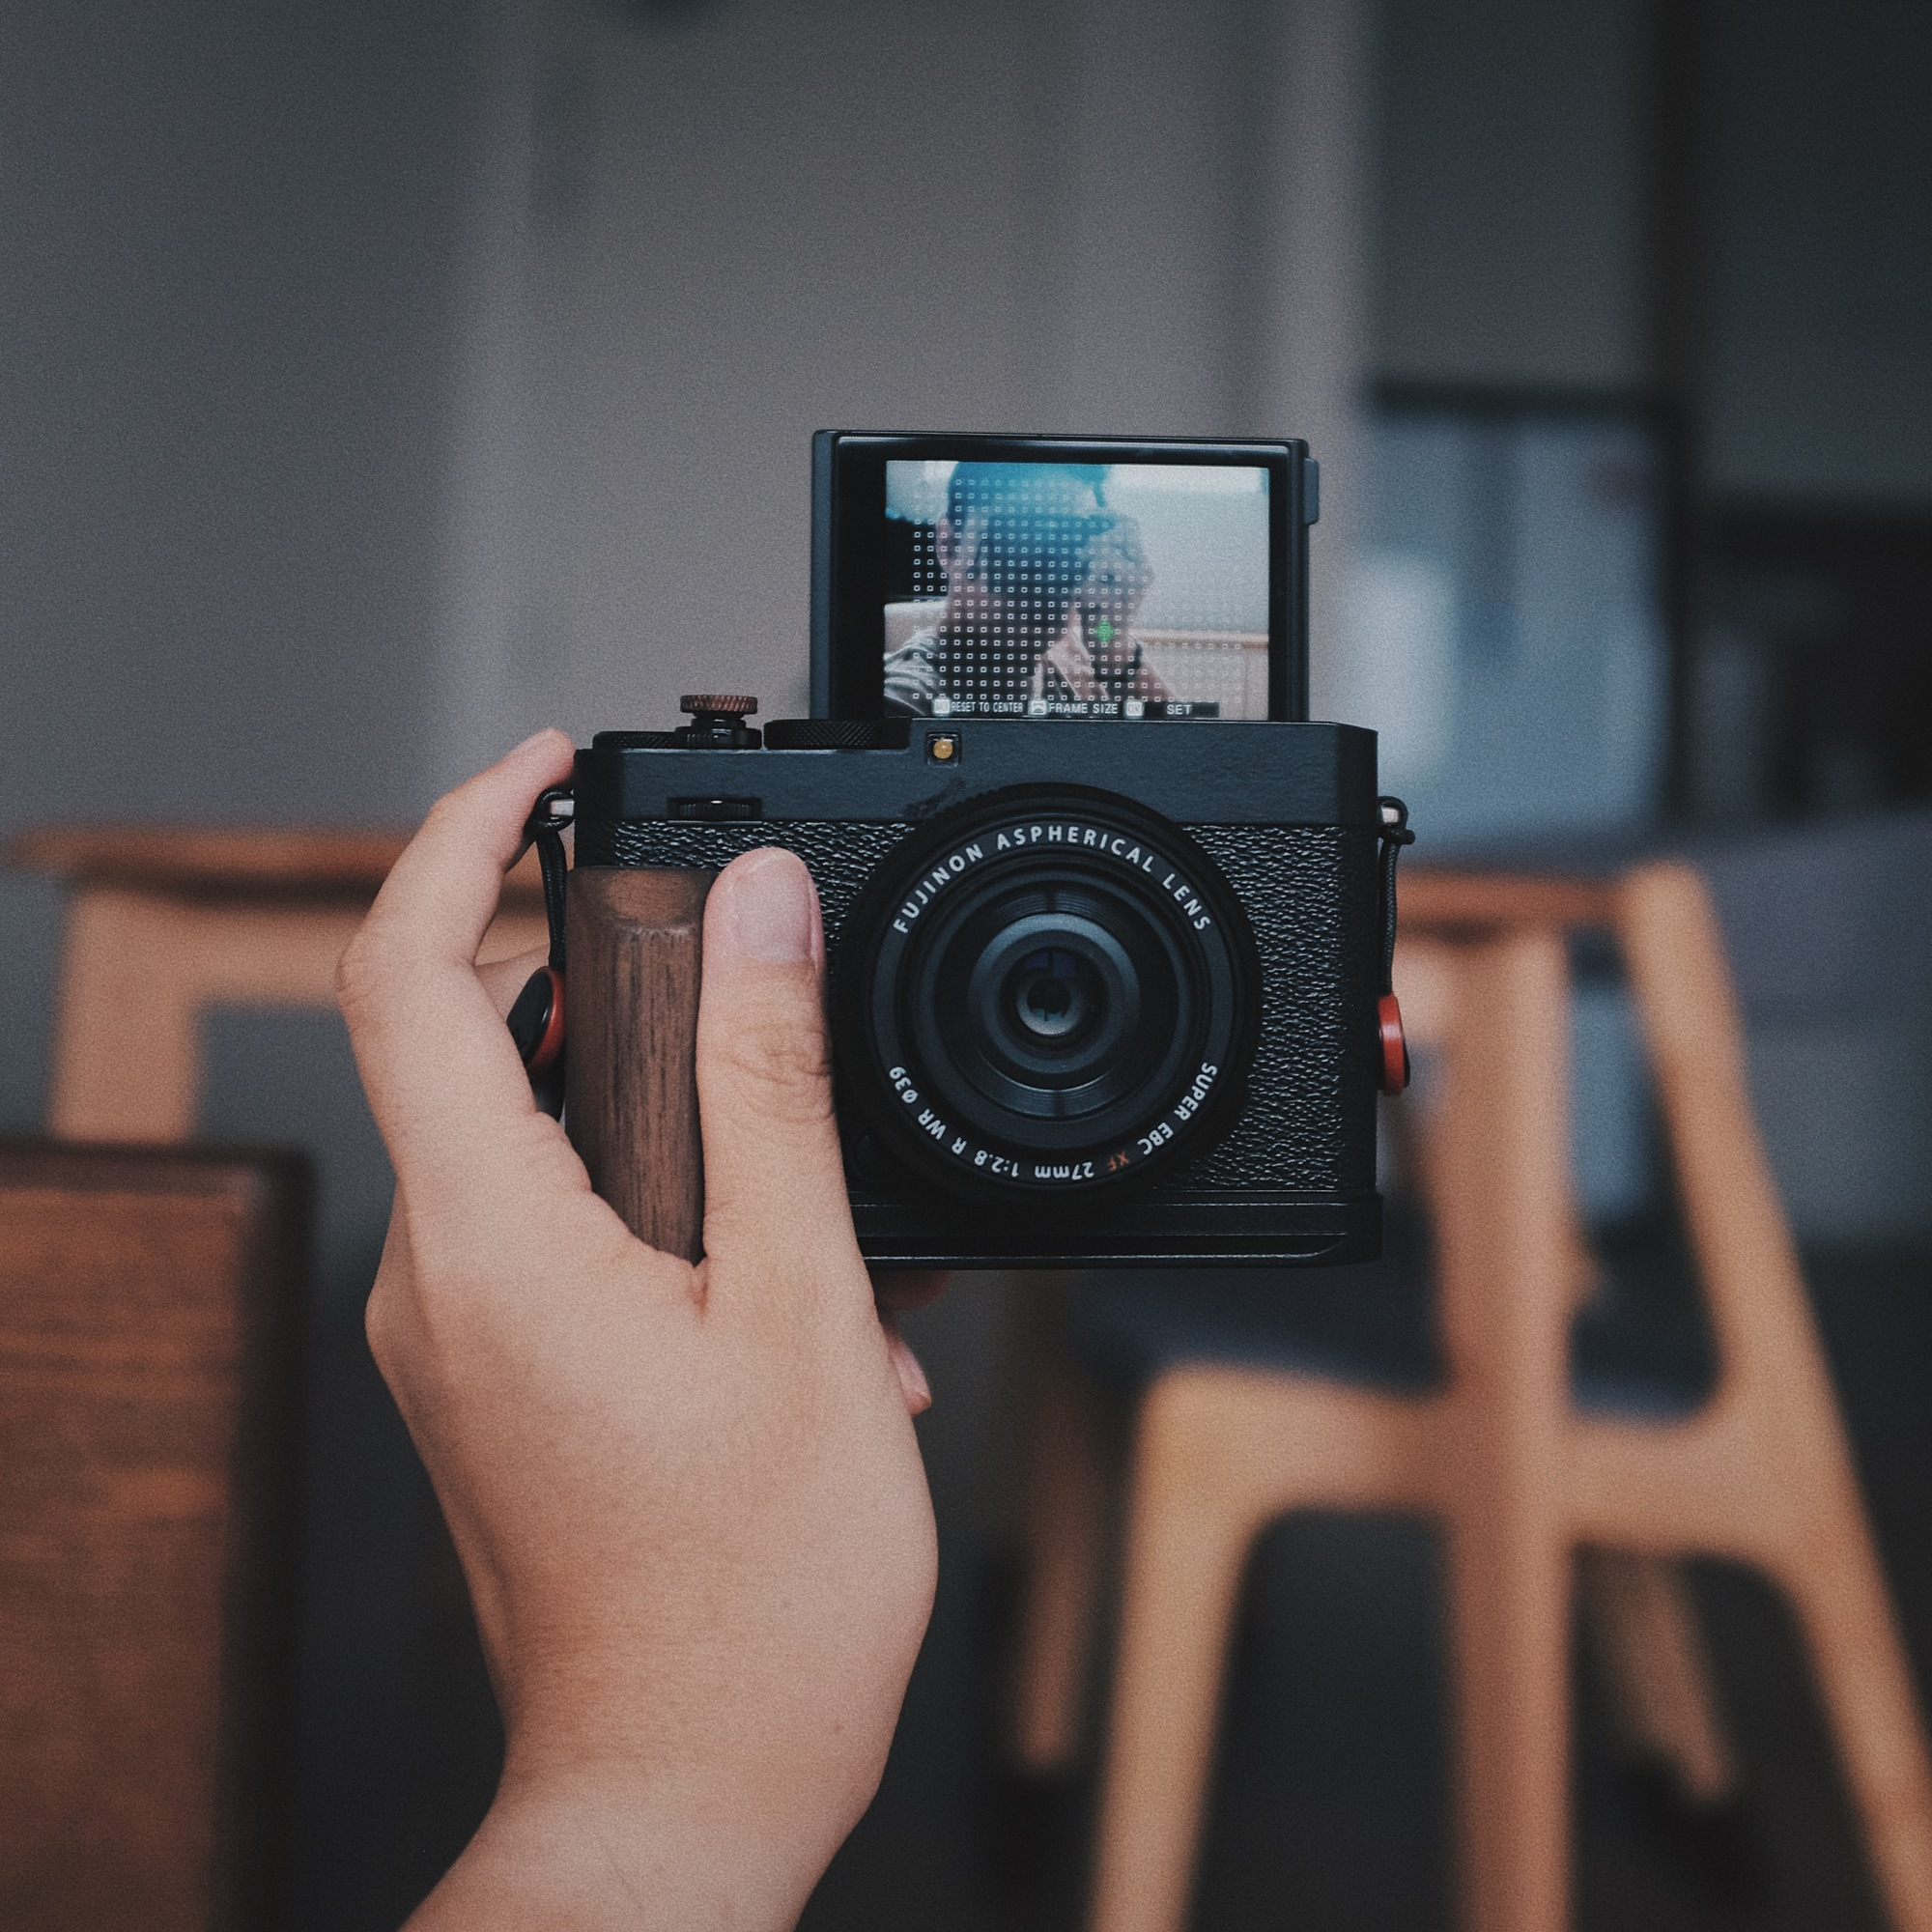
\includegraphics[width=\linewidth]{\envfinaldir/coverpic-prod.jpg}\par
            % \vskip 30pt
            \vfill

            \normalsize\rmfamily\scshape
            \copyright{} The Web Digest Project \hfill\large \envdatestr
        \end{center}
    \end{titlepage}
    % \restoregeometry
}
\newcommand{\simplehref}[1]{%
    \textcolor{blue!80!green}{\href{#1}{#1}}%
}
\renewcommand{\contentsname}{\center\Huge\sffamily\bfseries Contents\par\vskip 20pt}
\newcounter{ipartcounter}
\setcounter{ipartcounter}{0}
\newcommand{\ipart}[1]{
    % \vskip 20pt
    \clearpage
    \stepcounter{ipartcounter}
    \phantomsection
    \addcontentsline{toc}{chapter}{#1}
    % \begin{center}
    %     \Huge
    %     \sffamily\bfseries
    %     #1
    % \end{center}
    % \vskip 20pt plus 7pt
}
\newcounter{ichaptercounter}
\setcounter{ichaptercounter}{0}
\newcommand{\ichapter}[1]{
    % \vskip 20pt
    \clearpage
    \stepcounter{ichaptercounter}
    \phantomsection
    \addcontentsline{toc}{section}{\numberline{\arabic{ichaptercounter}}#1}
    \begin{center}
        \Huge
        \sffamily\bfseries
        #1
    \end{center}
    \vskip 20pt plus 7pt
}
\newcommand{\entrytitlefont}[1]{\subsection*{\raggedright\Large\sffamily\bfseries#1}}
\newcommand{\entryitemGeneric}[2]{
    % argv: title, url
    \parbox{\linewidth}{
        \entrytitlefont{#1}\par\vskip 5pt
        \footnotesize\ttfamily\mdseries
        \simplehref{#2}
    }\vskip 11pt plus 11pt minus 1pt
}
\newcommand{\entryitemGithub}[3]{
    % argv: title, url, desc
    \parbox{\linewidth}{
        \entrytitlefont{#1}\par\vskip 5pt
        \footnotesize\ttfamily\mdseries
        \simplehref{#2}\par\vskip 5pt
        \small\rmfamily\mdseries#3
    }\vskip 11pt plus 11pt minus 1pt
}
\newcommand{\entryitemAp}[3]{
    % argv: title, url, desc
    \parbox{\linewidth}{
        \entrytitlefont{#1}\par\vskip 5pt
        \footnotesize\ttfamily\mdseries
        \simplehref{#2}\par\vskip 5pt
        \small\rmfamily\mdseries#3
    }\vskip 11pt plus 11pt minus 1pt
}
\newcommand{\entryitemHackernews}[3]{
    % argv: title, hnurl, rawurl
    % \parbox{\linewidth}{
    %     \entrytitlefont{#1}\par\vskip 5pt
    %     \footnotesize\ttfamily\mdseries
    %     \simplehref{#3}\par
    %     \textcolor{black!50}{\href{#2}{#2}}
    % }\vskip 11pt plus 11pt minus 1pt
    \begin{minipage}{\linewidth}
            \entrytitlefont{#1}\par\vskip 5pt
            \footnotesize\ttfamily\mdseries
            \simplehref{#3}\par
            \textcolor{black!50}{\href{#2}{#2}}
    \end{minipage}\par\vskip 11pt plus 11pt minus 1pt
}







\begin{document}

\makeheader

\tableofcontents\clearpage




\ipart{Developers}
\ichapter{Hacker News}
\entryitemTwoLinks{I am rich and have no idea what to do}{https://news.ycombinator.com/item?id=42579873}{https://vinay.sh/i-am-rich-and-have-no-idea-what-to-do-with-my-life/}

\entryitemTwoLinks{iTerm2 critical security release}{https://news.ycombinator.com/item?id=42579472}{https://iterm2.com/downloads/stable/iTerm2-3\_5\_11.changelog}

\entryitemTwoLinks{Advent of Code 2024 in pure SQL}{https://news.ycombinator.com/item?id=42577736}{http://databasearchitects.blogspot.com/2024/12/advent-of-code-2024-in-pure-sql.html}

\entryitemTwoLinks{Tell HN: Impassable Cloudflare challenges are ruining my browsing experience}{https://news.ycombinator.com/item?id=42577076}{https://news.ycombinator.com/item?id=42577076}

\entryitemTwoLinks{TinyStories: How Small Can Language Models Be and Still Speak Coherent English? (2023)}{https://news.ycombinator.com/item?id=42576755}{https://arxiv.org/abs/2305.07759}

\entryitemTwoLinks{uBlock Origin GPL code being stolen by team behind honey browser extension}{https://news.ycombinator.com/item?id=42576443}{https://old.reddit.com/r/uBlockOrigin/comments/1hr6xjc/ubo\_quick\_filters\_list\_being\_stolen\_by\_team/}

\entryitemTwoLinks{XiangShan – open-source high performance RISC-V processor}{https://news.ycombinator.com/item?id=42576242}{https://github.com/OpenXiangShan/XiangShan}

\entryitemTwoLinks{Diagnosing an Unusual WiFi Issue (2020)}{https://news.ycombinator.com/item?id=42575990}{https://ryuuta.net/blog/diagnosing-an-unsual-wifi-issue/}

\entryitemTwoLinks{Postgres UUIDv7 and per-back end monotonicity}{https://news.ycombinator.com/item?id=42575900}{https://brandur.org/fragments/uuid-v7-monotonicity}

\entryitemTwoLinks{Ask HN: Who is hiring? (January 2025)}{https://news.ycombinator.com/item?id=42575537}{https://news.ycombinator.com/item?id=42575537}

\entryitemTwoLinks{Ask HN: Who wants to be hired? (January 2025)}{https://news.ycombinator.com/item?id=42575535}{https://news.ycombinator.com/item?id=42575535}

\entryitemTwoLinks{What Is miniKanren?}{https://news.ycombinator.com/item?id=42574125}{http://minikanren.org/}

\entryitemTwoLinks{Ask HN: Where to Work After 40?}{https://news.ycombinator.com/item?id=42573875}{https://news.ycombinator.com/item?id=42573875}

\entryitemTwoLinks{MitmProxy2Swagger: Automagically reverse-engineer REST APIs}{https://news.ycombinator.com/item?id=42572662}{https://github.com/alufers/mitmproxy2swagger}

\entryitemTwoLinks{Ray Tracing in One Weekend}{https://news.ycombinator.com/item?id=42572602}{https://raytracing.github.io/books/RayTracingInOneWeekend.html}

\entryitemTwoLinks{Standard Ebooks Public Domain Day 2025 in Literature}{https://news.ycombinator.com/item?id=42572573}{https://standardebooks.org/blog/public-domain-day-2025}

\entryitemTwoLinks{Dropbox Engineering Career Framework}{https://news.ycombinator.com/item?id=42572515}{https://dropbox.github.io/dbx-career-framework/}

\entryitemTwoLinks{Zasper: A Modern and Efficient Alternative to JupyterLab, Built in Go}{https://news.ycombinator.com/item?id=42572057}{https://github.com/zasper-io/zasper}

\entryitemTwoLinks{Autodesk deletes old forum posts suddenly}{https://news.ycombinator.com/item?id=42571995}{https://forums.autodesk.com/t5/net/regarding-community-content-archiving/td-p/13198106}

\entryitemTwoLinks{Mercure: A WebSocket alternative for server-sent events}{https://news.ycombinator.com/item?id=42571651}{https://github.com/dunglas/mercure}\ichapter{Phoronix}
\entryitemGeneric{\hskip 0pt{}Patches Proposed To Begin Plumbing 32-bit LoongArch CPU Support For The Linux Kernel}{https://www.phoronix.com/news/LoongArch-32-bit-Linux-uAPI}

\entryitemGeneric{\hskip 0pt{}32 Patches Merged For More Unification Between RadeonSI OpenGL \& RADV Vulkan Drivers}{https://www.phoronix.com/news/RADV-RadeonSI-Unify-In-Lowering}

\entryitemGeneric{\hskip 0pt{}Linux Patches Updated For Experimental Arm Morello That Combines Arm + CHERI ISA}{https://www.phoronix.com/news/Arm-Morello-Linux-v3}

\entryitemGeneric{\hskip 0pt{}Linux Prepares AMD "SRSO\_USER\_KERNEL\_NO" Support For Zen 5 CPUs}{https://www.phoronix.com/news/AMD-Linux-SRSO\_USER\_KERNEL\_NO}

\entryitemGeneric{\hskip 0pt{}Fedora Stakeholders Talk Of Forking Intel's Compute Runtime To Maintain Older Hardware}{https://www.phoronix.com/news/Intel-CR-Legacy-Possible-Fork}

\entryitemGeneric{\hskip 0pt{}AMD Zen 5 Captivated Linux Reader Interest In 2024}{https://www.phoronix.com/news/2024-Most-Popular-Reviews}

\entryitemGeneric{\hskip 0pt{}Lenovo Gaming Series WMI Drivers Updated For Enabling Extra Functionality Under Linux}{https://www.phoronix.com/news/Lenovo-Gaming-Series-Drivers-v2}

\entryitemGeneric{\hskip 0pt{}ACD Power/Performance Feature Being Worked On For The GPU Within The Snapdragon X1}{https://www.phoronix.com/news/Snapdragon-X1-Adreno-ACD}

\entryitemGeneric{\hskip 0pt{}Linux "steelseries" Driver Being Extended For The SteelSeries Arctis 9 Wireless Headset}{https://www.phoronix.com/news/SteelSeries-Arctis-9-Linux}


\ipart{Developers~~~~(zh-Hans)}
\ichapter{Solidot}
\entryitemGeneric{\hskip 0pt{}无聊的城市建筑不利于你的健康}{https://www.solidot.org/story?sid=80221}

\entryitemGeneric{\hskip 0pt{}人体组织中的微塑料与特定疾病相关}{https://www.solidot.org/story?sid=80220}

\entryitemGeneric{\hskip 0pt{}小米修改了引导程序解锁政策}{https://www.solidot.org/story?sid=80219}

\entryitemGeneric{\hskip 0pt{}美国南方几乎都屏蔽了 Pornhub }{https://www.solidot.org/story?sid=80218}

\entryitemGeneric{\hskip 0pt{}因 Windows 11 24H2 Bug 刺客信条起源在 Steam 平台遭遇差评轰炸}{https://www.solidot.org/story?sid=80217}

\entryitemGeneric{\hskip 0pt{}四分之三的 Steam Linux 用户使用 AMD CPU}{https://www.solidot.org/story?sid=80216}

\entryitemGeneric{\hskip 0pt{}阿里巴巴因竞争激烈对其大模型降价 85\%}{https://www.solidot.org/story?sid=80215}

\entryitemGeneric{\hskip 0pt{}2024 年 X.Org Server 的开发活跃度达到 10 年来的峰值}{https://www.solidot.org/story?sid=80214}

\entryitemGeneric{\hskip 0pt{}如果人类不会说话他们的集体认知可能不如蚂蚁}{https://www.solidot.org/story?sid=80213}

\entryitemGeneric{\hskip 0pt{}2024 年比亚迪全球销量 427 万辆}{https://www.solidot.org/story?sid=80212}

\entryitemGeneric{\hskip 0pt{}大力水手、丁丁以及更多米老鼠动画进入公有领域}{https://www.solidot.org/story?sid=80211}

\entryitemGeneric{\hskip 0pt{}diaspora*项目七成流量来自 AI 机器人}{https://www.solidot.org/story?sid=80209}

\entryitemGeneric{\hskip 0pt{}中端智能手机销量大幅下滑}{https://www.solidot.org/story?sid=80208}

\entryitemGeneric{\hskip 0pt{}《师父(SIFU )》在 Epic Games Store 限免 }{https://www.solidot.org/story?sid=80207}

\entryitemGeneric{\hskip 0pt{}天文学家利用韦伯望远镜发现烛龙螺旋星系}{https://www.solidot.org/story?sid=80206}

\entryitemGeneric{\hskip 0pt{}AI 数据中心影响美国居民的电力质量}{https://www.solidot.org/story?sid=80205}

\entryitemGeneric{\hskip 0pt{}中国计划 2025 年在戈壁滩建造钍基熔盐反应堆}{https://www.solidot.org/story?sid=80204}

\entryitemGeneric{\hskip 0pt{}黑客从地面劫持和修复 Beesat-1 立方体卫星}{https://www.solidot.org/story?sid=80203}

\entryitemGeneric{\hskip 0pt{}中国原油需求可能提前达到峰值}{https://www.solidot.org/story?sid=80202}

\entryitemGeneric{\hskip 0pt{}特斯拉用持 H-1B 签证的外国工人取代被裁的美国员工}{https://www.solidot.org/story?sid=80201}\ichapter{V2EX}
\entryitemGeneric{\hskip 0pt{}[职场话题] 国外的工作环境是怎么样的?也有办公室政治吗?}{https://www.v2ex.com/t/1102167}

\entryitemGeneric{\hskip 0pt{}[问与答] 请教下哪里可以方便写小作文?}{https://www.v2ex.com/t/1102166}

\entryitemGeneric{\hskip 0pt{}[问与答] 2025 新年迷思 毫无意义的深漂打工何时结束}{https://www.v2ex.com/t/1102165}

\entryitemGeneric{\hskip 0pt{}[酷工作] [远程,实习或全职] Python 编程及儿童编程机器人编程开发实习生}{https://www.v2ex.com/t/1102164}

\entryitemGeneric{\hskip 0pt{}[问与答] 淘宝买 pixel 手机问题求解}{https://www.v2ex.com/t/1102163}

\entryitemGeneric{\hskip 0pt{}[问与答] 公司后端比前端、测试、产品地位低正常吗?后端 10 人、测试 5 人、前端(web adnorid ios)10 人。}{https://www.v2ex.com/t/1102162}

\entryitemGeneric{\hskip 0pt{}[问与答] 用鼠标,你们用哪个手指滑动滚轮?我用的中指}{https://www.v2ex.com/t/1102161}

\entryitemGeneric{\hskip 0pt{}[Apple] 为什么 android 双微信可以, ios 就不行?}{https://www.v2ex.com/t/1102160}

\entryitemGeneric{\hskip 0pt{}[问与答] 市面上现在有没有 windows 系统同步当前浏览的网页金额收藏夹以及系统安装的软件及工具的工具,最好是开源的}{https://www.v2ex.com/t/1102159}

\entryitemGeneric{\hskip 0pt{}[程序员] 一种不付费使用 cursor 的方式}{https://www.v2ex.com/t/1102158}

\entryitemGeneric{\hskip 0pt{}[iOS] 大佬们, ios 自带输入法的自动遗忘用户词库的毛病是普遍性的还是我个人问题?能否彻底改善?}{https://www.v2ex.com/t/1102157}

\entryitemGeneric{\hskip 0pt{}[Debian] debian12.8 的 preseed 自动安装方式,封装 iso 的正确方式??}{https://www.v2ex.com/t/1102156}

\entryitemGeneric{\hskip 0pt{}[FFmpeg] 使用 FFmpeg 试图做个人用的转码点播服务端, 但 mpegts 多个切片间音频偶尔不连续?}{https://www.v2ex.com/t/1102154}

\entryitemGeneric{\hskip 0pt{}[问与答] 如果有人给钱让你做公司法人你做不做,看了深圳工商局宣传视频 受诱骗登记商事主体 并非都可以撤销登记}{https://www.v2ex.com/t/1102153}

\entryitemGeneric{\hskip 0pt{}[分享创造] 2025 年新上线的 smm+ai 工具站。。。}{https://www.v2ex.com/t/1102152}

\entryitemGeneric{\hskip 0pt{}[NAS] NAS 上如何批量管理 RAW+JPG 照片?}{https://www.v2ex.com/t/1102149}

\entryitemGeneric{\hskip 0pt{}[Telegram] 大家有啥经常看的 telegram 频道推荐订阅?}{https://www.v2ex.com/t/1102148}

\entryitemGeneric{\hskip 0pt{}[问与答] 求效果最好的长篇文章中英互译工具}{https://www.v2ex.com/t/1102147}

\entryitemGeneric{\hskip 0pt{}[职场话题] 自勉:降低心理预期,继续坚持继续面}{https://www.v2ex.com/t/1102144}

\entryitemGeneric{\hskip 0pt{}[问与答] 碰到个难搞的 dns 更新问题, 咨询下域控大佬}{https://www.v2ex.com/t/1102142}

\entryitemGeneric{\hskip 0pt{}[成都] 豆豉烤鱼成都哪家推荐一下}{https://www.v2ex.com/t/1102141}

\entryitemGeneric{\hskip 0pt{}[分享发现] 浙里办 App(iOS)的用户代理}{https://www.v2ex.com/t/1102140}

\entryitemGeneric{\hskip 0pt{}[问与答] 三文鱼不是深水鱼为什么能生吃?}{https://www.v2ex.com/t/1102139}

\entryitemGeneric{\hskip 0pt{}[分享创造] 打卡 21 天计划, Build In Public 21 Days}{https://www.v2ex.com/t/1102138}

\entryitemGeneric{\hskip 0pt{}[V2EX] 请问访问 V2EX 时不时提示 Attention Required! Cloudflare,该怎么解决?}{https://www.v2ex.com/t/1102137}

\entryitemGeneric{\hskip 0pt{}[分享发现] 2025 年 1 月,盈透美股账户尚能开通,附开通攻略和邀请链接}{https://www.v2ex.com/t/1102136}

\entryitemGeneric{\hskip 0pt{}[问与答] v0.dev 开发的 Next.js 项目,下载代码到本地,怎么跑起来?}{https://www.v2ex.com/t/1102135}

\entryitemGeneric{\hskip 0pt{}[成都] 成都有线下 AI 入门学习课程或者讲座一类的吗}{https://www.v2ex.com/t/1102134}

\entryitemGeneric{\hskip 0pt{}[问与答] 入职互联网企业 2 个月,薪水谈低了,我打算去搞一把}{https://www.v2ex.com/t/1102133}

\entryitemGeneric{\hskip 0pt{}[问与答] 农村老家过年有什么好的活动吗? 往年都是烧烤}{https://www.v2ex.com/t/1102132}

\entryitemGeneric{\hskip 0pt{}[分享发现] 热心的 V 友们,碰到诈骗电话和钓鱼网站怎么举报了}{https://www.v2ex.com/t/1102131}

\entryitemGeneric{\hskip 0pt{}[程序员] 国内外均可访问的收费视频网站开发方案咨询}{https://www.v2ex.com/t/1102130}

\entryitemGeneric{\hskip 0pt{}[宽带症候群] 上海联通今晚怎么了?到上海电信延迟直接爆表}{https://www.v2ex.com/t/1102129}

\entryitemGeneric{\hskip 0pt{}[投资] 分享一个美股大盘云图}{https://www.v2ex.com/t/1102128}

\entryitemGeneric{\hskip 0pt{}[游戏开发] 我是如何从零开始手搓一个独立游戏并上架 Steam 的}{https://www.v2ex.com/t/1102126}

\entryitemGeneric{\hskip 0pt{}[分享创造] 开源一个胖东来,自油爱的小脚本。}{https://www.v2ex.com/t/1102125}

\entryitemGeneric{\hskip 0pt{}[分享创造] 肝了一个月-AI 图像视频生成网站-欢迎免费试用}{https://www.v2ex.com/t/1102124}

\entryitemGeneric{\hskip 0pt{}[问与答] Chrome 干翻 IE 算不算个奇迹}{https://www.v2ex.com/t/1102122}

\entryitemGeneric{\hskip 0pt{}[问与答] 如何将 iPhone 中的 QQ 聊天记录完整迁移到 Mac?}{https://www.v2ex.com/t/1102121}

\entryitemGeneric{\hskip 0pt{}[Android] 周经贴,求推荐手机,预算 2800-3200}{https://www.v2ex.com/t/1102120}

\entryitemGeneric{\hskip 0pt{}[iPhone] ios9 在 2025 年已经几乎不能用了}{https://www.v2ex.com/t/1102117}

\entryitemGeneric{\hskip 0pt{}[生活] 好东西最先吃还是最后吃的问题}{https://www.v2ex.com/t/1102116}

\entryitemGeneric{\hskip 0pt{}[广州] 广州天河有那种可以短租一两个月的酒店吗?}{https://www.v2ex.com/t/1102115}

\entryitemGeneric{\hskip 0pt{}[5G] 各位帝都的兄弟们,北京移动 5G 网络在室内的速度难道就是这样的吗?}{https://www.v2ex.com/t/1102114}

\entryitemGeneric{\hskip 0pt{}[问与答] 浪潮 gs 这个能搭建单机环境么?}{https://www.v2ex.com/t/1102113}

\entryitemGeneric{\hskip 0pt{}[宽带症候群] 有一个疑惑,为何家庭宽带上行带宽应用被跑满后,下行带宽应用可能就无法使用了?}{https://www.v2ex.com/t/1102112}

\entryitemGeneric{\hskip 0pt{}[职场话题] 太难了,谈薪越定越低}{https://www.v2ex.com/t/1102111}

\entryitemGeneric{\hskip 0pt{}[问与答] 想问问有没有一个电脑同时安装多个网银的办法。}{https://www.v2ex.com/t/1102110}

\entryitemGeneric{\hskip 0pt{}[优惠信息] pikpak 合租 黑五特价 5 人人均 30.8}{https://www.v2ex.com/t/1102108}

\entryitemGeneric{\hskip 0pt{}[Apple] 苹果播客的网页版无法加载,即使开了全局美国的代理?}{https://www.v2ex.com/t/1102107}


\ipart{Generic News}
\ichapter{联合早报}
\entryitemWithDescription{沈泽玮:台湾冲突阻遏法案只叫不咬?}{https://www.zaobao.com/news/china/story20240918-4758889}{美国众议院9月9日开启了长达一星期的``中国周'',共通过25项主要涉华法案。(法新社) 美国众议院在当地时间9月9日开启了长达一星期的``中国周'',在美国总统和国会选举举行之前,密集表决数十项与中国有关的法案,共通过25项主要涉华法案……}

\entryitemWithDescription{欧盟电动车关税投票倒计时 中国在分歧中寻支持}{https://www.zaobao.com/news/china/story20240917-4758953}{欧盟27个成员国将于9月25日就是否继续对进口自中国的电动汽车额外征税进行最后表决。图为上海港等待装运出口的电动汽车。(彭博社) 欧盟对中国电动汽车加征关税的投票进入倒计时,正在欧洲访问的中国商务部部长王文涛与欧盟多国政府高层就此进行协商,试图在立场分歧的成员国中争取到更多支持。 受访学者研判,欧盟对中国电动汽车加征关税不可避免,但具体的加税方式和幅度仍有一定弹性,这是王文涛此行与各国谈判的重点……}

\entryitemWithDescription{港府今年将举办逾400项国庆活动}{https://www.zaobao.com/news/china/story20240917-4759341}{再过十多天就是中国国庆75周年,香港天星小轮展示``国庆75周年''\,``三天免费搭小轮''等标语迎国庆。(中新社) 再过十多天就是中国国庆75周年,香港特区政府今年将举办逾400项庆祝活动,希望通过一连串活动庆祝国庆,并且弘扬爱国主义教育及刺激消费。 港府星期二(9月17日)召开记者会,介绍各项庆祝国庆活动和特别优惠,涉及出行及吃喝玩乐等领域……}

\entryitemWithDescription{美空军部长:中国大陆军演精密化 为入侵封锁台湾做准备}{https://www.zaobao.com/news/china/story20240917-4759407}{美国空军部长肯德尔星期一(9月16日)在空军暨太空军协会的一场大会上致辞,提到中国对印太地区日益增长的威胁。(取自美国国防部网站) (华盛顿综合讯)美国空军部长肯德尔指,中国大陆军演的规模越来越大,也更加精密化,这是在专门为入侵、封锁台湾做准备。他也称,中国对印太地区的威胁现在已存在……}

\entryitemWithDescription{批准潜在对台备件军售案后 美派巡逻机过航台海}{https://www.zaobao.com/news/china/story20240917-4758770}{台军士兵8月26日在屏东县枋山训练场进行实弹演习时,从M1167 TOW运载车上发射一枚美制TOW-2A线导反坦克导弹。(路透社) (华盛顿/台北/北京综合讯)在批准潜在对台备件军售案之后,美国派遣反潜巡逻机过航台湾海峡,中国人民解放军东部战区则组织战机跟监美机,并誓言``坚决捍卫国家主权''……}

\entryitemWithDescription{李家超:若香港驻美经贸办被关 受害的是美企}{https://www.zaobao.com/news/china/story20240917-4758797}{香港特首李家超星期一(9月17日)警告,如果美国通过法案,导致香港驻美经贸办关闭,受害的是美国企业。图为李家超9月11日在``一带一路''高峰论坛上致辞。(彭博社) (香港综合讯)香港特首李家超警告,如果美国通过法案,导致香港驻美经贸办关闭,受害的是美国企业。 美国众议院上周通过《香港经济贸易办事处认证法案》,如果参议院也表决通过并交由总统签署成法,香港三个驻美国的经贸办可能将被强制关闭……}

\entryitemWithDescription{美国指中国航空工业集团员工企图实施黑客攻击}{https://www.zaobao.com/news/china/story20240917-4757988}{(华盛顿综合讯)中国航空航天巨头中国航空工业集团一名员工被指试图对美国宇航局、美国军方和其他目标展开黑客攻击。 据彭博社报道,美国检察官布坎南星期一(9月16日)在起诉书中,指控中国航空工业集团39岁的工程师吴宋(音译,Song Wu)企图从美国宇航局、空军、陆军和海军,以及联邦航空管理局取得电脑软件和源代码……}

\entryitemWithDescription{【东谈西论】恒大账务造假 普华永道是共犯还是被拖累?}{https://www.zaobao.com/news/china/story20240917-4756452}{因涉及恒大地产审计项目的违法行为,普华永道中国9月13日被中国财政部和证监会处以4.41亿人民币罚款并被令停业六个月, 广州分所被撤销……}

\entryitemWithDescription{戴庆成:香港输入人才计划大检阅}{https://www.zaobao.com/news/china/story20240917-4744978}{香港于2022年底推出高端人才通行证计划。(法新社) 2019年香港反修例风波过后,数以十万计港人移居海外,令香港出现人才荒。港府为了解决这个问题,在过去几年积极引入``新血'',当中以高才通计划最受瞩目,社会上也不时热议其成效。 高才通全称为高端人才通行证计划,于2022年底推出,申请人年收入须达到250万港元(约42万新元)以上,或本科毕业于全球百强大学并满足一定工作年限等……}

\entryitemWithDescription{中美希望稳定双边关系 中小国家可​​​搭建桥梁}{https://www.zaobao.com/news/china/story20240917-4745091}{中美元首去年11月在旧金山会晤后,双方都希望稳定两国关系,我国巡回大使陈庆珠认为,如果中美两国都认为走向战争不符合它们的利益,那么中小国家就可以做点什么,为双方搭建桥梁。 陈庆珠星期一(9月16日)在李光耀公共政策学院的一场研讨会上说,中国与西方的关系面对诸多困难,有中国智库表示,希望新加坡能协助在中美之间建立更多对话,``因为新加坡受美国信任,也在中国有渠道''……}

\entryitemWithDescription{陈庆珠:世界经历了三次``中国冲击'' 中美的主导力之争将继续}{https://www.zaobao.com/news/china/story20240917-4744996}{李光耀公共政策学院``思想之节庆''的一场研讨会,讨论``历史终结时的中国冲击''。左起是我国巡回大使陈庆珠、通商中国主席李奕贤、李光耀公共政策学院国际关系助理教授何莉菁、李光耀公共政策学院院长柯成兴……}

\entryitemWithDescription{上海遭遇75年来最强台风 扰乱民众中秋假期出行}{https://www.zaobao.com/news/china/story20240916-4745224}{台风贝碧嘉星期一(9月16日)登陆上海,维护人员星期一下午在衡山路上处理倒伏的树木。 (新华社) 台风造成上海上万株数目倒伏或折断。图为一棵倒下的大树砸坏一旁的建筑。(法新社) 台风贝碧嘉登陆上海后,黄浦江苏州河口潮位上涨,乌云密布。(中新社) 中国上海市星期一(9月16日)遭遇75年来最强台风``贝碧嘉''登陆,也是上海有记录以来首次有强台风侵袭……}

\entryitemWithDescription{陆男频长驱偷渡台湾在测试边防实力?}{https://www.zaobao.com/news/china/story20240916-4745161}{中国大陆一名王姓男子在中秋节前夕,乘橡皮艇从浙江宁波抵达台湾新北市林口,主动打电话投案,海巡署人员前去接他上岸。(自由時報) 中国大陆一名王姓男子划橡皮艇于上星期六清晨偷渡到台湾,隔天被新北市地方法院裁定羁押禁见。这是6月以来第二起大陆人士偷渡至台湾,此间专家质疑是否为海防破口,并怀疑对岸是否在测试台湾的边防实力……}

\entryitemWithDescription{中美时隔八月举行国防部工作会晤}{https://www.zaobao.com/news/china/story20240916-4745025}{(北京/华盛顿综合讯)中美双方上周末举行国防部工作会晤;美国官员称,美国积极进行美中两军外交活动,不代表美国对有关中国议题的处理方式发生任何改变。 据中国国防部星期天(15日)晚上通报,北京香山论坛结束后,第18次中美国防部工作会晤上星期六至星期天(9月14日至15日)在北京举行……}

\entryitemWithDescription{中国高校今年拟增足球运动本科专业}{https://www.zaobao.com/news/china/story20240916-4744925}{(北京综合讯)为了培养足球专业人才,中国大专学府今年度拟新增足球运动本科专业,以具体落实中国足球改革。 综合人民网和《南方都市报》报道,中国教育部上星期五(9月13日)发布《2024年度普通高等学校本科专业申报材料公示》。根据公示统计,今年度拟新增专业535个,涉及353所高校,其中39所高校新增足球运动专业……}

\entryitemWithDescription{香港23条首案 港男因穿``光时''上衣被定罪}{https://www.zaobao.com/news/china/story20240916-4743439}{(香港综合讯)香港一名无业男子,今年6月因穿印有2019年反修例抗争口号的上衣而被捕。他星期一承认违反煽动意图罪,成为在《维护国家安全条例》(即《香港基本法》第23条)下被定罪的第一人。 综合港媒《星岛日报》和路透社报道,27岁无业男子诸启邦今年6月12日在石门港铁站附近,未能出示身份证供查阅被警方拘捕……}

\entryitemWithDescription{美国务院:中国释放被关押近20年美籍牧师}{https://www.zaobao.com/news/china/story20240916-4744614}{(华盛顿综合电)中国释放被关押近20年的美国籍牧师,显示北京在中美关系的关键时刻展现善意。 综合彭博社、法新社和路透社报道,美国国务院发言人星期天(9月15日)说:``我们欢迎林大卫(音译,David Lin)从中华人民共和国的监狱获释。他已回返美国,这是他近20年来首次与家人见面。'' 林大卫的女儿艾丽斯告诉美国政治新闻网Politico,她的父亲将抵达得克萨斯州的圣安东尼奥……}

\entryitemWithDescription{中国驻泰使馆:近期并未向湄公河下游泄洪}{https://www.zaobao.com/news/china/story20240916-4743917}{(北京讯)泰国西北部的湄公河因洪水泛滥而决堤,中国否认这是中方泄洪所致,并称近来已持续减少云南景洪水电站的出库流量,以助下游地区抗洪。 中国驻泰国大使馆星期日(9月15日)深夜在官方微信公众号发文说,当天又有媒体报道称中国正在向湄公河泄洪,经向中国主管部门核实,使馆再次澄清,为帮助下游地区应对洪灾,中方近来持续稳定和减少景洪水电站出库流量,不可能对下游地区抗洪救灾形成压力……}

\entryitemWithDescription{加入美国储存可靠度评估计划 台湾军方编列预算采购三类型导弹}{https://www.zaobao.com/news/china/story20240916-4743826}{(台北讯)据台媒报道,台湾军方持续向美国采购可简易操作的导弹,预计在2024年、2031年以前获得400枚``标枪''反装甲导弹、2485枚``刺针''人携式防空导弹……}

\entryitemWithDescription{韩咏红:中美分头追逐全球南方}{https://www.zaobao.com/news/china/story20240916-4730719}{9月5日,中国外长王毅(中)同中非合作论坛非方现任共同主席国塞内加尔外长法勒(左)、下任共同主席国刚果外长加科索(右),在北京共同会见中外记者并答问。(路透社) 进入气候宜人的9月,中国接连举行了两场受瞩目的国际会议,一是聚集非洲53国国家元首与政要的中非合作论坛,接着是周末刚闭幕的北京香山论坛。 两场活动的参与者不同,规模也有很大差距……}

\entryitemWithDescription{菲律宾船只撤离中菲争议海域后 将再派船接替}{https://www.zaobao.com/news/china/story20240915-4730494}{这张在9月15日拍摄,并由菲律宾海岸警卫队提供的照片显示,菲律宾海岸警卫队船马格巴努亚号抵达了菲国巴拉望岛的一个港口。菲律宾早前以发现填海活动为由,今年4月派出马格巴努亚号前往萨比纳礁。(法新社/菲律宾海岸警卫队) 菲律宾国家海事委员会星期天(9月15日)发声明称,该国海岸警卫队一艘巡逻舰已离开萨比纳礁争议海域……}

\entryitemWithDescription{台风贝碧嘉直击中国华东 多趟本地与沪杭间航班取消}{https://www.zaobao.com/news/china/story20240915-4730611}{9月15日在上海外滩滨江步道上,一名外籍游客的雨伞被大风吹起。台风贝碧嘉的中心当天下午5时位于上海市东偏南方大约435公里的东海海面上,中心附近最大风力有13级。(中新社) (上海/新加坡综合讯)台风贝碧嘉预计将为中国华东沿海地区带来狂风暴雨,多趟往返新加坡与上海和杭州的航班取消……}






\clearpage
\leavevmode\vfill
\footnotesize

Copyright \copyright{} 2023-2025 Neruthes and other contributors.

This document is published with CC BY-NC-ND 4.0 license.

The entries listed in this newsletter may be copyrighted by their respective creators.

This newsletter is generated by the Web Digest project.

The newsletters are also delivered via Telegram channel \CJKunderline{\href{https://t.me/webdigestchannel}{https://t.me/webdigestchannel}}.\\
RSS feed is available at \CJKunderline{\href{https://webdigest.pages.dev/rss.xml}{https://webdigest.pages.dev/rss.xml}}.

This newsletter is available in PDF at
\CJKunderline{\href{https://webdigest.pages.dev/}{https://webdigest.pages.dev/}}.

The source code being used to generate this newsletter is available at\\
\CJKunderline{\href{https://github.com/neruthes/webdigest}{https://github.com/neruthes/webdigest}}.

This newsletter is also available in
\CJKunderline{\href{http://webdigest.pages.dev/readhtml/\envyear/WebDigest-20250103.html}{HTML}} and
\CJKunderline{\href{https://github.com/neruthes/webdigest/blob/master/markdown/\envyear/WebDigest-20250103.md}{Markdown}}.


\coverpic{https://unsplash.com/photos/a-man-and-a-woman-are-smiling-for-the-camera-rERcszlmrcM}{Ellery Sterling}


\end{document}
